\documentclass[12pt,a4paper,hidelinks]{article}

\usepackage{ulem}
\usepackage{incgraph}
\usepackage{tikz}
\usepackage{hyperref}

\newcommand{\leftcoordinate}{-15cm}
\usetikzlibrary{mindmap,shadows,calendar,fadings}
\tikzset{todo/.append style={annotation,above,concept color=white,draw=black,text width=2cm,align=center}}
\hypersetup{
    colorlinks=false,
    linkcolor=black,
    filecolor=magenta,      
    urlcolor=cyan,
}

\begin{document}
\begin{inctext}
    \begin{tikzpicture}
        \pgfdeclarelayer{background}
        \pgfdeclarelayer{foreground}
        \pgfsetlayers{background,main,foreground}
        % ------------------------ declare mindmap ------------------------ %
        \begin{scope}[
                mindmap,
                grow cyclic,
                concept color=red!60!green!100!blue!20,
                every node/.append style={concept,circular drop shadow},
                level 1/.append style={sibling angle=360/5}
            ]
            \node[root concept, fill=white](skyrim){
                \href{../game.pdf}{SKYRIM}
            }
            child{
                    node{
                            SKSE
                        }
                }
            ;
        \end{scope}
        % ------------------------ background ------------------------ %
        \begin{pgfonlayer}{background}
            \node{
                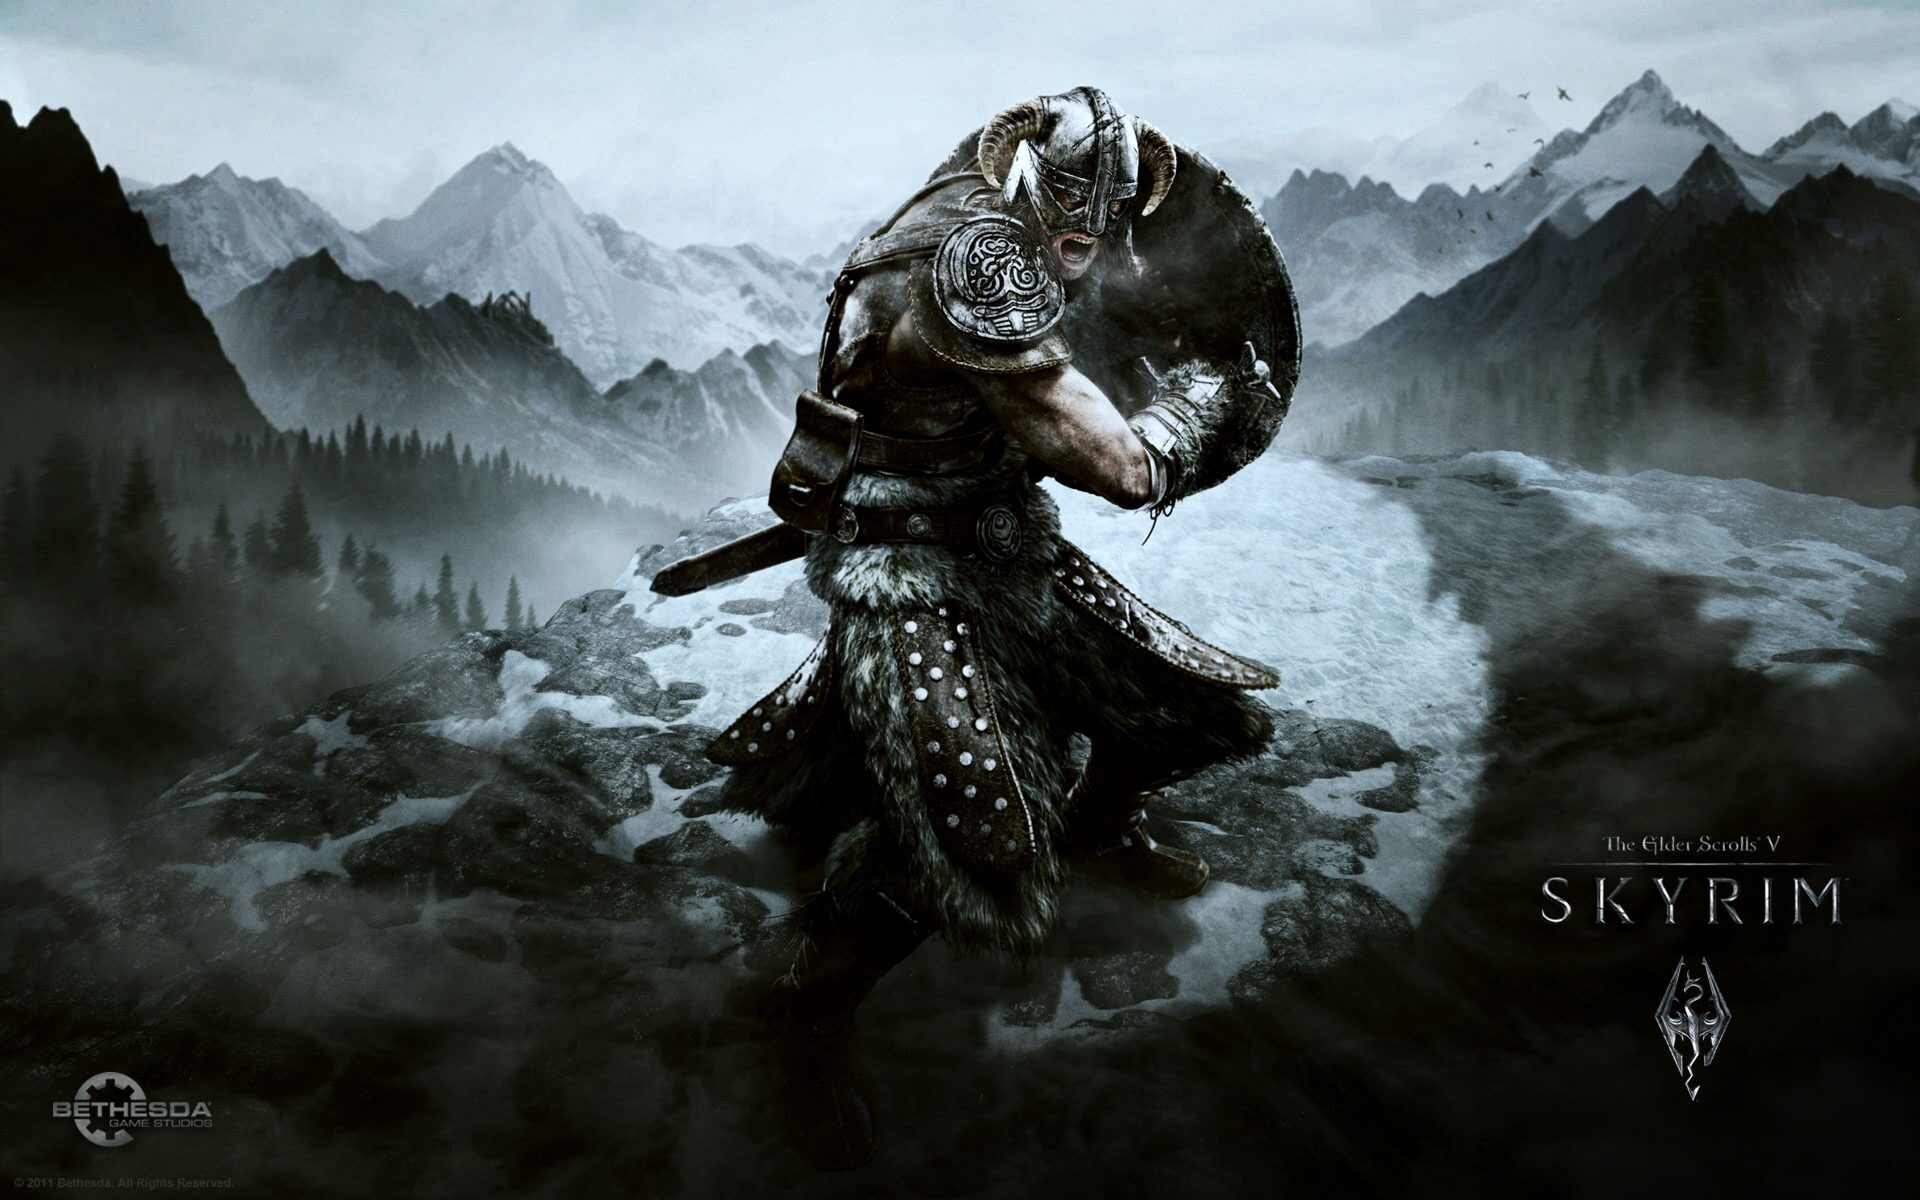
\includegraphics[width=\paperwidth]{../../../image/skyrim.jpeg}
            };
        \end{pgfonlayer}
        % ------------------------ foreground ------------------------ %
        \begin{pgfonlayer}{foreground}
            \node[text width=1.3cm, text height=1.3cm,yshift=-1.1cm] at (skyrim) {
                \href{run:../../../mindmap.pdf}{
\includegraphics[width=1.3cm,height=1.3cm]{../../../image/skyrim2.png}}
            };
        \end{pgfonlayer}
    \end{tikzpicture}
\end{inctext}
%------------------------------------------------------------ List ------------------------------------------------------------%
\newpage
\end{document}